\chapter{Aplicația desktop}

\section{Simulator de particule}
Aplicația desktop este un simulator interactiv de particule în care utilizatorul poate acționa asupra acestora prin definirea unui punct pe un plan 2D, care se comportă ca un centru gravitațional. Simulatorul oferă o reprezentare vizuală intuitivă a mișcării particulelor, permițând experimentarea cu diferite valori pentru a crea niște efecte vizuale cât mai spectaculoase. Punctul de atracție gravitațională este stabilit în funcție de poziția mouse-ului, iar forța gravitațională este activată doar atunci când utilizatorul apasă butonul stâng al mouse-ului. În momentul în care butonul nu mai este acționat, atracția punctului este dezactivată, iar particulele își continuă mișcarea sub influența inerției. 

Pentru a facilita interacțiunea utilizatorului cu parametrii utilizați de simulator, dar și pentru a vedea rezultatele acestuia, aplicația integrează o interfață grafică intuitivă care permite monitorizarea și configurarea parametrilor. Interfața este compusă dintr-un meniu principal, reprezentat ca o bara orizontală în partea de sus a ferestrei, și încă două ecrane separate: \textit{Settings} și \textit{GPU Metrics}. Meniul principal este acționat folosind tasta \texttt{ALT}, iar pentru celalalte două ferestre se pot folosi shortcut-urile \texttt{CTRL+E} pentru \textit{Settings}, respectiv \texttt{CTRL+C} pentru \textit{GPU Metrics}. Fereastra \textit{Settings}, oferă control asupra parametrilor fundamentali ai simulării. Utilizatorul poate regla numărul total de particule redate și schema de culori utilizată pentru vizualizarea lor. Există două tipuri de culori: o culoare statică, reprezentând particulele în repaus, cu viteză minimă sau nulă, și o culoare dinamică, reprezentând particulele în mișcare, cu viteză crescută. Fereastra \textit{GPU Metrics}, oferă informații detaliate despre performanța aplicației. Acesta afișează următoarele metrici: numele plăcii video utilizate, rata de cadre pe secundă (FPS) alături de un grafic de evoluție, timpul de procesare pentru un singur cadru (Frame Time) măsurat în milisecunde vizualizat folosind un grafic corespunzător, precum și statistici legate de FPS: FPS mediu, FPS minim și FPS maxim. Toate aceste metrici sunt calculate pe baza ultimelor 4096 de cadre randate, oferind o perspectivă relevantă asupra performanței sistemului. Graficul pentru vizualizarea timpului de procesare pe cadru a fost adaptat după următorul articol \cite{FrameTimesVisualization_citation}. Fiecare cadru din secvența graficului este reprezentat printr-un dreptunghi codificat vizual: culoarea indică performanța, lățimea este raportată la durata de timp a cadrului, iar înălțimea evidențiază diferențele relevante de timp între oricare două cadre succesive. Ferestrele destinate interacțiunii cu utilizatorul pot fi acționate separat, în afara contextului Vulkan de rendering. Toate funcționalitățile interfeței au fost construite cu ajutorul bibliotecii externe ImGui \cite{ImGui_citation}, care oferă mai multe instrumente pentru a dezvolta într-un mod ușor și eficient interfețe vizuale. 

Pentru a evalua performanța aplicației într-un mod sistematic și ușor de reprodus, este implementat un sistem de benchmark automat. Acesta execută teste predefinite cu inputuri standardizate salvate sub forma unui fișier cu formatul \textit{\texttt{.json}}, ceea ce va permite o analiză obiectivă a performanței pe diferite configurații hardware și sisteme de operare. În acest fișier sunt definite valorile corespunzătoare coordonatelor poziției mouse-ului și acționării butonului stâng al mouse-ului, împreună cu un timestamp cu ajutorul căruia este specificat momentul în care trebuie trimise evenimentele, astfel încât să fie recepționate de aplicație. Există cinci teste predefinite care pot fi efectuate folosind opțiunea de benchmark din meniul principal, dar pot fi modificate în orice moment pentru a acoperi alte scenarii de testare atât timp cât este respectat formatul prestabilit. Pentru a simplifica și pentru a respecta automat formatul necesar fișierului de intrare \textit{\texttt{.json}}, a fost introdusă opțiunea de capta istoricul evenimentelor pe care le-a generat un utilizator. Acest instrument poate fi activat/oprit direct din meniul principal, secțiunea \textit{Tools}, opțiunea \textit{Capture Input}, sau prin folosirea shortcut-ului \texttt{CTRL+R}. Rezultatul va fi salvat în fișierul \textit{\texttt{auto-capture.json}} în momentul în care este oprită înregistrarea. Valorile colectate pot fi modificate și utilizate ulterior pentru a crea un nou test de benchmark personalizat. Pentru a putea lucra cu formatul \textit{\texttt{.json}} este integrată biblioteca externă header only, nlohmann \cite{nlohmann-json_citation} gândită pentru dezoltarea aplicațiilor care doresc în implementarea lor o abordare C++ modernă. 

% TODO
% \begin{figure}[ht]
%     \centering
%     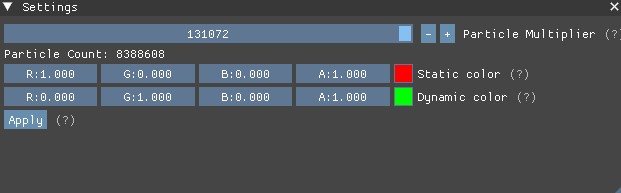
\includegraphics[width=0.8\textwidth]{images/settings-window.jpg}
%     \caption{Fereastra \textit{Settings}}
%     \label{fig:settings-window}
% \end{figure}

% ============================================================================================================
\section{Vulkan API}
% ============================================================================================================
Vulkan este un API modern de randare și computație, dezvoltat de Khronos Group \cite{KhronosGroup_citation}, care oferă control low-level asupra GPU-ului. Spre deosebire de API-uri mai vechi precum OpenGL, Vulkan este conceput pentru a minimiza overhead-ul driver-ului, ceea ce oferă o gestionare mai eficientă a resurselor hardware și permite totodată, optimizarea semnificativă a performanței, reducând latențele și îmbunătățind viteza de execuție. Filosofia din spatele API-ului Vulkan se bazează pe oferirea unui control aproape complet asupra GPU-ului, permițând dezvoltatorilor să obțină performanță maximă \cite{VulkanPhilosophy_citation}. Totuși, acest nivel ridicat de control vine cu complexitate sporită, deoarece API-ul necesită gestionarea manuală a fiecărui aspect low-level ce ține de interacțiunea cu placa video, de la modul în care sunt gestionate alocarea resurselor, până la sincronizarea dintre CPU si GPU. Dezvoltatorii trebuie să fie foarte expliciți la etapele de creare și configurare a pipeline-urilor grafice, ordinea comenzilor de rendering și la gestionarea memoriei tuturor buffers create. 

Am optat pentru Vulkan datorită performanței superioare și a flexibilității pe care o oferă în comunicarea cu placa video. Printre avantajele cheie care au condus la alegerea acestui API se numără: suportul avansat pentru multi-threading; gestionarea explicită a memoriei; pipeline grafic personalizabil. În primul rând, suportul avansat pentru multi-threading permite distribuirea sarcinilor grafice și de computație pe mai multe fire de execuție, reducând astfel blocajele și maximizând utilizarea resurselor disponibile. Aplicația se folosește de acestă componentă prin execuția unui \textit{compute shader}, ce are ca scop distribuirea sarcinilor pe mai multe nuclee și thread-uri ale plăcii video. În al doilea rând, gestionarea explicită a memoriei, permite programatorilor să controleze direct alocarea, eliberarea și reutilizarea spațiului în VRAM. Această abordare reduce overhead-ul asociat cu managementul automat al memoriei și oferă posibilitatea de a optimiza cu exactitate granularitatea transferurilor de date și alocarea resurselor, aspecte critice pentru minimizarea fragmentării și maximizarea coerenței cache-ului. Acest proces reduce operațiile de transfer redundante, permițând dezvoltatorilor să evite copierile inutile de date între memoria RAM și memoria VRAM, fapt ce duce la scăderi semnificative ale timpului de procesare și ale necesarului de lățime de bandă. Acestă idee este explorată în simulator prin folosirea de \textbf{\mintinline{latex}{Push Constants}} și \textbf{\mintinline{latex}{Uniform Buffer Objects}}. În același timp, această abordare permite reutilizarea zonelor de memorie pentru diferite resurse, cum ar fi reutilizarea unui buffer pentru multiple etape de procesare sau pentru obiecte temporare, maximizând astfel eficiența utilizării VRAM și reducând necesitatea alocării dinamice de memorie. Conceptul este implementat prin folosirea unui \textbf{\mintinline{latex}{Shader Storage Buffer Object}}, un buffer prezent și utilizat atât în etapa definită de \textit{compute shader}, cât și în cea de \textit{vertex shader}. În plus, Vulkan permite crearea unui pipeline grafic personalizabil, oferind dezvoltatorilor control complet asupra etapelor de procesare grafică. Acest lucru elimină operațiile inutile din driver și permite optimizări avansate, cum ar fi utilizarea layout-urilor optimizate sau reducerea schimbărilor redundante de stare. Nu în ultimul rând, Vulkan oferă un control avansat al sincronizării între CPU și GPU, asigurând coerența datelor și prevenind conflictele de acces la resurse comune. Acest control este realizat prin mecanisme precum semafoare, bariere de memorie și fences, care permit coordonarea precisă a comenzilor și reducerea timpilor de așteptare.

Deși Vulkan este un API scris în limbajul C, am ales să folosesc C++ pentru dezvoltarea aplicației datorită combinației sale de performanță ridicată, control manual asupra memoriei și suportului avansat pentru programarea orientată pe obiecte. C++ oferă mecanisme puternice de gestionare a resurselor prin intermediul paradigmei RAII (Resource Acquisition Is Initialization) \cite{RAII_citation}, un principiu fundamental care asigură că resursele alocate sunt eliberate automat atunci când obiectele care le dețin ies din contextul de operare, evitând astfel \textit{memory leaks} și alte erori legate de alocarea dinamică, frecvent întâlnite în limbajul C. 

% ============================================================================================================
\section{Arhitectura aplicației}
% ============================================================================================================
Arhitectura aplicației se bazează pe o implementare modulară și eficientă a sistemului de particule, care se folosește la capacitate maximă de proprietățile plăcii video. Sistemul de particule este proiectat astfel încât fiecare particulă să fie complet independentă, cu un set unic de date, ceea ce permite paralelizarea tuturor calculelor necesare unei singure instanțe prin intermediul unui \textit{compute shader}, responsabil pentru gestionarea și actualizarea proprietațiilor fiecărei particule, cum ar fi poziția și viteza, profitând în acest mod, de capacitățile de procesare paralelă ale arhitecturilor moderne de GPU. 

Această abordare exploatează pe deplin arhitectura paralelă masivă \cite{ParallelArchitectures_citation} (Massively Parallel Architecture) a unităților de procesare grafică, care au fost concepute special pentru a executa mii de operații și calcule simultan. Spre deosebire de unitățile centrale de procesare optimizate pentru execuția secvențială, plăcile video integrează mii de nuclee destinate unor calcule simple, fiecare capabil să proceseze independent seturi de date. Acest ecosistem computațional specializat permite manipularea eficientă a volumelor mari de date omogene, prin distribuirea uniformă a sarcinii de calcul pe toate nucleele fizice disponibile. Astfel, fiecare particulă beneficiază de resurse dedicate de procesare, eliminând blocajele de performanță specifice arhitecturilor secvențiale. Un alt aspect care justifică alegerea acestei soluții este dat de faptul că între procesoarea oricăror două particule nu este necesar niciun mecanism de așteptare, nu există nicio formă de comunicare sau schimb de date între două instanțe de particule, fiecare având proprietățile calculate într-un mediu complet izolat, fără să țină cont de datele altor particule din sistem. 

Pentru vizualizarea rezultatelor sistemului de particule, este necesară crearea unui context grafic și a unei ferestre în care placa de video să poată afișa conținutul. Această funcționalitate este implementată folosind biblioteca GLFW (Graphics Library Framework) \cite{GLFW_citation}, care oferă un API modular și eficient pentru gestionarea ferestrelor, contextului Vulkan, configurarea suprafețelor de redare și prelucrarea evenimentelor de intrare (tastatură, mouse, controller). O altă blibliotecă externă care a fost integrată este GLM (OpenGL Mathematics) \cite{GLM_citation}, o bibliotecă C++ header only care oferă un set complet de tipuri și funcții matematice esențiale pentru dezvoltarea unei aplicații grafice, precum operații cu vectori, matrici, transformări geometrice (translație, rotație, scalare) și calcul de proiecții (ortografică, perspectivă). 

Alegerea fizică a dispozitivului grafic optim reprezintă o etapă importantă în configurarea aplicației, deoarece performanța și stabilitatea sistemului de particule depind în mod direct de capacitățile hardware ale unității de procesare grafică. În majoritatea sistemelor moderne, sunt disponibile două categorii de dispozitive grafice. În prima categorie se regăsesc plăcile video integrate, care sunt incorporate direct în procesorul central și utilizează memoria RAM, iar în a doua categorie sunt plăcile video dedicate, echipate cu memoria video proprie (VRAM), fiind special proiectate pentru sarcini de calcul intensiv. Această selecție joacă un rol esențial deoarece va avea cel mai mare impact în determinarea performanței și a capacităților de calcul ale aplicației. Diferențele dintre o placă video integrată și una dedicată pot duce la diferențe uriașe în aplicațiile solicitante din punct de vedere grafic. Pentru a asigura compatibilitatea și performanța maximă, aplicația implementează un mecanism de selecție manuală a GPU-ului, care enumeră toate dispozitivele grafice disponibile în sistem și formează o ierahie ce reflectă performanța acestora, fiind evaluate conform unui set de criterii tehnice predefinite. Vom alege device-ul cu cele mai multe și rapide nuclee disponibile pentru calculul paralel. De asemnea, este necesar să aibă abilitatea de a prezenta imaginile rezultate în urma întregului proces computațional. O altă cerință este suportul pentru extensiile obligatorii de care are nevoie sistemul de particule, printre care se regăsesc \textit{\texttt{VK\_KHR\_swapchain}}, \textit{\texttt{VK\_KHR\_storage\_buffer\_storage\_class}}. În contextul unui simulator de particule, care solicită o putere de calcul paralelă cât mai mare, utilizarea unei plăci video dedicate este preferată. 

În arhitectura API-ului Vulkan, conceptele de queue families și queues joacă un rol crucial în gestionarea execuției operațiilor pe GPU. Acestea sunt în esență structuri care controlează fluxul de comenzi trimise de CPU către GPU. Fiecare GPU expune una sau mai multe Queue Families, fiecare specializată în anumite tipuri de operații. În contextul unui simulator de particule, aplicația necesită acces la două tipuri de cozi: \textit{graphics queue} și \textit{compute queue}, utilizate pentru execuția celor două pipeline-uri specializate. \textit{Graphics Queue} este folosită pentru procesul de rendering al particulelor pe ecran, ceea ce include desenare, blending, rasterization, execuția de vertex și fragment shaders. \textit{Compute Queue} este folosită pentru a executa operații în paralel, ceea ce include calcularea și actualizarea proprietăților particulelor. Acestă componentă a API-ului este extrem de eficientă în manipularea volumelor mari de date și în execuția rapidă a algoritmilor matematici necesari pentru simularea realistă a mișcării particulelor. 

\textit{Swap chain} (lanțul imaginilor pregătite pentru afișare) este mecanismul central în Vulkan pentru gestionarea imaginilor prezentate pe ecran. Acesta constă într-o colecție de buffers, de obicei două sau trei, care alternează între stările de afișare și rendering, asigurând o experiență fluidă. Pentru a îmbunătăți calitatea procesului de rendering, este utilizată o imagine temporară numită \textit{Intermediary Image}, care are un nivel mai mare de multisampling, fiecare pixel este eșantionat de 8 ori. Tehnica \textit{Multisampling Anti-Aliasing} \cite{MSAA_citation} (MSAA) reduce artefactele de la marginile obiectelor desenate, îmbunătățind calitatea imaginii procesate. După ce imaginea intermediară este procesată, aceasta este transpusă în imaginea din swap chain, numită \textit{Swap Chain Image}, utilizată pentru prezentarea finală în fereastra aplicației. 

% ============================================================================================================
\section{Buffers}
% ============================================================================================================
Sistemul de particule dezvoltat în cadrul acestui proiect utilizează trei tipuri principale de buffere pentru a gestiona eficient datele între CPU și GPU: \textbf{\mintinline{latex}{Uniform Buffers}}, \textbf{\mintinline{latex}{Push Constants}} și \textbf{\mintinline{latex}{Shader Storage Buffer Object}}. Alegerea acestor tipuri de buffere a fost ghidată de nevoia de a maximiza performanța și de a minimiza latențele de transfer. 

% Uniform Buffers
\vspace{1em}
\begin{wrapfigure}{r}{0.5\textwidth}
\vspace{-1em}
\hspace{1.2cm}
\begin{minipage}{\linewidth}
\begin{minted}[escapeinside=||, linenos=true]{cpp}
struct UniformBufferObject
{
    |\color[HTML]{b00040}\textbf{glm::mat4}| projection;
    |\color[HTML]{b00040}\textbf{glm::vec4}| staticColor;
    |\color[HTML]{b00040}\textbf{glm::vec4}| dynamicColor;
};
\end{minted}
\end{minipage}
\vspace{-1em}
\end{wrapfigure}

\indent{\textbf{\mintinline{latex}{Uniform Buffers Objects}}} sunt folosite pentru a stoca date care nu se schimbă frecvent. Aceste buffers sunt preferate într-un context în care este nevoie de o modalitate eficientă și simplă de a partaja date constante între CPU și GPU, fără a consuma excesiv lățimea de bandă a memoriei. Pentru a permite accesul CPU-ului la aceste date, obiectele buffer sunt create astfel încât să fie vizibile atât pentru procesor, cât și pentru placa video. Pentru aplicația implementată, am ales să folosesc acest tip de buffer pentru a stoca matricea de proiecție și culorile folosite în colorarea particulelor deoarece sunt valori actualizate foarte rar, posibil să rămână constante pe tot parcursul derulării simulatorului. Matricea de proiecție este actualizată doar când sunt schimbate dimensiunile ferestrei principale, iar cele două culori pot fi modificate doar la comanda utilizatorului. 

% Push Constants
\vspace{1em}
\begin{wrapfigure}{l}{0.5\textwidth}
\vspace{-1em}
\hspace{1.5cm}
\begin{minipage}{\linewidth}
\begin{minted}[escapeinside=||, linenos=true]{cpp}
struct PushConstants
{
    uint32_t enabled;
    float timestep;
    |\color[HTML]{b00040}\textbf{glm::vec2}| attractor;
};
\end{minted}
\end{minipage}
\vspace{-1em}
\end{wrapfigure}

\indent{\textbf{\mintinline{latex}{Push Constants}}} sunt în esență un alt mecanism de transmitere a datelor, care oferă o metodă extrem de rapidă de a furniza valori mici și frecvent actualizate către shaders. Spre deosebire de \textbf{\mintinline{latex}{Uniform Buffer Objects}}, care necesită alocare explicită, gestionare a memoriei și un set de \textit{binding descriptors}, acestea sunt inserate direct în pipeline-ul grafic și transmise prin comenzile de rendering, eliminând overhead-ul asociat transferurilor de date. Conform documentației \cite{PushConstantsSizeLimits_citation}, Vulkan garantează cel puțin 128 bytes pentru capacitatea unui bloc de date tip \textbf{\mintinline{latex}{Push Constants}}. O cerință importantă de care trebuie ținut cont în construcția unei structuri \textbf{\mintinline{latex}{Push Constants}} este să respecte regulile formatului SPIR-V pentru offset și stride \cite{Offset-and-Stride-Assignment_citation}. Dimensiunea primitivelor \textbf{\mintinline[escapeinside=||]{latex}{uint32|\textcolor{black}{\_}|t}} și \textbf{\mintinline{latex}{float}} este de 4 bytes, prin urmare trebuie aliniate în memorie la un multiplu de 4 bytes, iar \textbf{\mintinline{latex}{glm::vec2}} are 8 bytes, așa că trebuie aliniat la un mulitplu de 8 bytes. O modalitate de a organiza datele necesare astfel încât se fie respectate regulile enunțate și să aibă cel mai compact mod de a reprezenta toate cele 3 variabile, este cel definit în structura \textbf{\mintinline{latex}{PushConstants}}, ilustrată în \autoref{fig:push-constants}. Acestă structură păstrează datele contiguu în memorie, fără să aibă goluri de memorie pe post de offset, asigurând coerența cache-ului și acces eficient. 

\begin{figure}
    \centering
    \includesvg[width=0.6\linewidth]{images/PushConstantsMemoryLayout.svg}
    \caption{Reprezentarea în memorie pentru \textbf{\mintinline{latex}{Push Constants}}}
    \label{fig:push-constants}
\end{figure}

% Shader Storage Buffer Object (SSBO)
\vspace{1em}
\begin{wrapfigure}{r}{0.5\textwidth}
\vspace{-1em}
\hspace{1.2cm}
\begin{minipage}{\linewidth}
\begin{minted}[escapeinside=||, linenos=true]{cpp}
struct Particle
{
    |\color[HTML]{b00040}\textbf{glm::vec2}| position;
    |\color[HTML]{b00040}\textbf{glm::vec2}| velocity;
};
\end{minted}
\end{minipage}
\vspace{-1em}
\end{wrapfigure}

Un \textbf{\mintinline{latex}{Shader Storage Buffer Object}} \textbf{\mintinline{latex}{(SSBO)}} este folosit pentru a gestiona volume mari de date care trebuie procesate exclusiv pe GPU. Acest tip de buffer este extrem de eficient în contextul unui simulator de particule deoarece permite stocarea directă a datelor în VRAM, ceea ce conferă plăcii video abilitatea de a efectua calculele instanțelor de particulă independent de CPU, reducând astfel latența asociată transferurilor de date. GPU-ul poate accesa aceste date la viteze mult mai mari decât ar fi posibil prin transferuri repetate între CPU și GPU. În cazul sistemului de particule, SSBO-ul va fi definit folosind datele specifice unei particule, reprezentate prin structura \textbf{\mintinline{latex}{Particle}}. Prima etapă în crearea datelor pentru acest buffer este generarea tututor valorilor de către CPU, urmată de transferul acestora către GPU. În esență, operația mută toate datele din memoria RAM în memoria VRAM. Odată transferate valorile inițiale ale particulelor de la CPU la GPU, placa video preia întreaga responsabilitate a actualizării lor. CPU-ul nu va mai avea niciun fel de acces, nu poate să citească sau să modifice în niciun fel datele din buffer, acesta devenind o resursă exclusivă a plăcii video. O caracteristică importantă a SSBO-urilor este că ele permit fiecărui fir de execuție al GPU-ului să acceseze independent datele particulelor, facilitând astfel paralelizarea masivă a calculelor. 

% ============================================================================================================
\section{Pipeline}
% ============================================================================================================
\begin{figure}[ht]
    \centering
    \includesvg[width=0.8\linewidth]{images/Pipeline.svg}
    \caption{Vulkan Pipeline (adaptare după figura din documentație \cite{VulkanPipeline_citation})}
    \label{fig:vulkan-pipeline}
\end{figure}

Codul implementează un flux de rendering în două etape distincte, exploatând pe cât de mult este posibil capabilitățile plăcii video pentru a maximiza performanța. În prima etapă, este folosit pipeline-ul de calcul (compute pipeline), care se ocupă de actualizarea stării particulelor. Acest prim pipeline folosește un \textit{compute shader}, cu ajutorul căruia procesează volume mari de date folosind mii de nuclee de calcul ale plăcii video, evitând astfel calculul lor pe CPU. Mutarea procesării datelor de simulare direct pe placa video aduce o îmbunătățire notabilă și performanțe foarte mari deoarece nu mai este necesară efectuarea mai multor transferuri costisitoare între memoria principală a CPU-ului și memoria GPU-ului. Astfel, toate datele rămân pe GPU, eliminând latențele asociate cu copierea datelor și permit o execuție paralelă în care sunt utilizate toate resursele hardware de care dispune placa video. În a doua etapă, este folosit pipeline-ul grafic (graphics pipeline), care realizează procesul de rendering a particulelor pe ecran. Acest pipeline este mai complex, incluzând mai mulți pași enumerați în \autoref{fig:vulkan-pipeline}. 

În \textit{compute shader} sunt calculate viteza și poziția fiecărei particule, folosind datele din \textbf{\mintinline{latex}{Push Constants}} referitoare la poziția și starea punctului de atracție, împreună cu ajutorul unui \textbf{\mintinline{latex}{Shader Storage Buffer Object}} în care sunt stocate datele actuale despre particule. Pe baza informațiilor primite, fiecare thread va actualiza valorile unei particule, poziția și viteza. \textit{Vertex shader} este responsabil de a lua datele din SSBO calculate în etapa anterioară, iar pe baza lor, împreună cu informațiile din \textbf{\mintinline{latex}{Uniform Buffer Object}}, determină culoarea și poziția în planul 2D specifice fiecărei particule. Nu în ultimul rând, \textit{fragment shader} atribuie fiecărei particule, ce se află în spațiul de rendering al ferestrei principale, culoarea calculată în vertex shader. 





% ============================================================================================================
% TODO: SCRIS
% ============================================================================================================
% - TODO: de spus mai in detaliu cum functioneaza partea de compute 
% - TODO: de explicat cum functioneaza in spate WARPS/ => video-urile cu compute
% - TODO: modul in care sunt compilate aceste shaders in formatul .spv + de ce se folosesc
% - TODO: de scris cum functioneaza formatul de shaders pentru Vulkan, cum si de ce sunt compilate, ce formate putem folosi care pot fi compilate in .spv